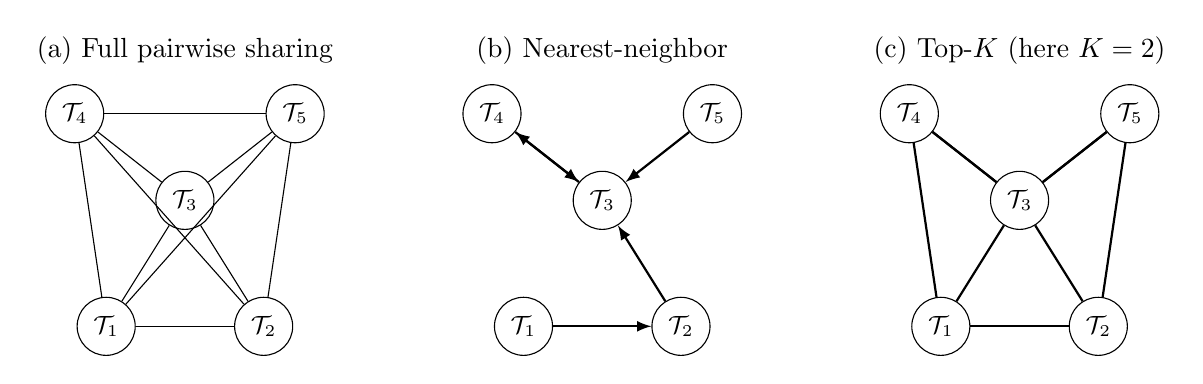
\begin{tikzpicture}[
    node/.style={circle, draw, minimum size=7mm, font=\small},
    >=latex,
    scale=1, every node/.style={transform shape}
]

% Positions (triangle + 2)
\node[node] (t1) at (0,0) {$\mathcal{T}_1$};
\node[node] (t2) at (2,0) {$\mathcal{T}_2$};
\node[node] (t3) at (1,1.6) {$\mathcal{T}_3$};
\node[node] (t4) at (-0.4,2.7) {$\mathcal{T}_4$};
\node[node] (t5) at (2.4,2.7) {$\mathcal{T}_5$};

% --- (a) Full sharing (left box) ---
\node at (1.0,3.5) {(a) Full pairwise sharing};

\draw (t1) -- (t2);
\draw (t1) -- (t3);
\draw (t1) -- (t4);
\draw (t1) -- (t5);

\draw (t2) -- (t3);
\draw (t2) -- (t4);
\draw (t2) -- (t5);

\draw (t3) -- (t4);
\draw (t3) -- (t5);

\draw (t4) -- (t5);

% --- (b) NN sharing (middle box) ---
\begin{scope}[xshift=5.3cm]
\node[node] (u1) at (0,0) {$\mathcal{T}_1$};
\node[node] (u2) at (2,0) {$\mathcal{T}_2$};
\node[node] (u3) at (1,1.6) {$\mathcal{T}_3$};
\node[node] (u4) at (-0.4,2.7) {$\mathcal{T}_4$};
\node[node] (u5) at (2.4,2.7) {$\mathcal{T}_5$};

\node at (1.0,3.5) {(b) Nearest-neighbor};

% Example NN edges (you can adapt per similarity):
\draw[->, thick] (u1) -- (u2);
\draw[->, thick] (u2) -- (u3);
\draw[->, thick] (u3) -- (u4);
\draw[->, thick] (u4) -- (u3);
\draw[->, thick] (u5) -- (u3);
\end{scope}

% --- (c) Top-K sharing (right box) ---
\begin{scope}[xshift=10.6cm]
\node[node] (v1) at (0,0) {$\mathcal{T}_1$};
\node[node] (v2) at (2,0) {$\mathcal{T}_2$};
\node[node] (v3) at (1,1.6) {$\mathcal{T}_3$};
\node[node] (v4) at (-0.4,2.7) {$\mathcal{T}_4$};
\node[node] (v5) at (2.4,2.7) {$\mathcal{T}_5$};

\node at (1.0,3.5) {(c) Top-$K$ (here $K=2$)};

% For K=2, connect each node to its 2 closest
\draw[thick] (v1) -- (v2);
\draw[thick] (v1) -- (v3);

\draw[thick] (v2) -- (v1);
\draw[thick] (v2) -- (v3);

\draw[thick] (v3) -- (v4);
\draw[thick] (v3) -- (v5);

\draw[thick] (v4) -- (v3);
\draw[thick] (v4) -- (v1);

\draw[thick] (v5) -- (v3);
\draw[thick] (v5) -- (v2);
\end{scope}

\end{tikzpicture}